%\documentclass[times, 10pt,twocolumn]{article}
\documentclass[times,10pt,onecolumn]{article}
\usepackage{latex8}
\usepackage{times}
\usepackage{algorithm}
\usepackage{algorithmic}
\usepackage{amssymb}
\usepackage{psfrag,graphicx}
\usepackage{doublespace}
\input{psfig.sty}
\pagestyle{empty}

\newenvironment{proof}[1][Proof]{\begin{trivlist}
\item[\hskip \labelsep {\bfseries #1}]}{\end{trivlist}}
\newenvironment{definition}[1][Definition]{\begin{trivlist}
\item[\hskip \labelsep {\bfseries #1}]}{\end{trivlist}}
\newenvironment{example}[1][Example]{\begin{trivlist}
\item[\hskip \labelsep {\bfseries #1}]}{\end{trivlist}}
\newenvironment{remark}[1][Remark]{\begin{trivlist}
\item[\hskip \labelsep {\bfseries #1}]}{\end{trivlist}}

\newcommand{\qed}{\nobreak \ifvmode \relax \else
      \ifdim\lastskip<1.5em \hskip-\lastskip
      \hskip1.5em plus0em minus0.5em \fi \nobreak
      \vrule height0.75em width0.5em depth0.25em\fi}

\newcommand{\prf}{\noindent{\textbf{Proof:}} }
\newcommand{\bbox}{\vrule height7pt width4pt depth1pt}
\newcommand{\eprf}{\bbox\vspace{0.1in}}

\newtheorem{theorem}{Theorem}[section]
\newtheorem{lemma}[theorem]{Lemma}
\newtheorem{proposition}[theorem]{Proposition}
\newtheorem{corollary}[theorem]{Corollary}
\newtheorem{heuristic}[theorem]{Heuristic}

\begin{document}

\setstretch{1}{
\title{Anonymous Network Protocol}

%\author{\hspace*{25pt} Wei-Shinn Ku$^{\S}$ \hspace*{1pt} and \hspace*{1pt} ???$^{\dag}$\\
%\hspace*{-200pt}\\
%\hspace*{20pt}{$^\S$Dept. of Computer Science and Software
%Engineering, Auburn University, Auburn, AL 36849} \\
%%\hspace*{20pt}{$^\dag$Department~of~Computer~Science, University , City 17590} \\
%\hspace*{20pt}{\texttt{\{weishinn@auburn.edu,???@.edu\}}}
%\\}

\maketitle

%\begin{abstract}
%In the participatory sensing, users with mobile devices (e.g. cell phones
%and laptop computers) participate in the collection of environmental
%information around them and submit the collected data to a central server
%for processing and analysis. Identity privacy of mobile users in this model
%is a major concern that hinders the adoption of this computing model. In
%this paper, we propose an anonymous networking protocol approach to protect
%the identity of part
%icipants of such computing model.
%\end{abstract}

%
In participatory
sensing~\cite{conf/sensys/ReddyBEHS07,conf/sensys/DuttaAKMMWW09},
users with mobile devices (e.g., cell phones with GPS chips)
participate in the collection of environmental information around
them and submit the collected data (image, audio, video, etc.) to
a central server for process, analysis, and
storage~\cite{DBLP:conf/mobisys/MunRSYBEHHWB09}. An example is the
OpenStreetMap~\cite{DBLP:journals/pervasive/HaklayW08} project,
which collects user contributed GIS data (such as GPS traces and
POIs) and constructs an online map, from mobile data, open for the
public to use. Other examples of participatory sensing include
cooperative collection of gas
prices~\cite{DBLP:conf/dcoss/DongKCB08}, monitoring of traffic
conditions~\cite{DBLP:conf/dcoss/ConceicaoFB08}, and photo sharing
through mobile applications such as Facebook and Instagram.

This model of ``crowd" data collection has many advantages due to
that the dynamic environmental data and information are quickly
captured by mobile users and disseminated to other users or to
central servers for analysis. Government censoring of information
is also less effective in this model since there could be many
mobile devices that are capturing the same event.

Despite the advantages, privacy of the users who contribute is a
major issue in participatory sensing and crowd-sourcing. Users may
not want to leak their locations with the contributed data lest
their movement should be
tracked~\cite{conf/icde/YiuJHL08,journals/pvldb/WangL09}. In the
case of controversial photos, a user may not want to reveal his or
her identity to the collection server (such as
WikiLeaks\footnote{http://wikileaks.org/}) since the user's
identity may be saved on the server and later uncovered by
government entities for prosecution. It is a fact that services on
the web collect user identifications along with the data submitted
by their users~\cite{wiki_privacy}. Even with websites, such as
Wikipedia\footnote{http://www.wikipedia.com} and
4chan\footnote{http://www.4chan.org/faq\#what4chan} that advertise
to be anonymous log IP addresses of contributors. Although an IP
address does not uniquely identify an individual, cellular data
service providers are required by law to keep record of assignment
of IP addresses to mobile users for a period of
time\footnote{http://uscode.house.gov/download/pls/18C121.txt}.
With an IP address, a piece of information stored on a server (be
it a photo, or a file) can be traced back to a user using the
technique discussed in~\cite{DBLP:journals/ijufks/Sweene02} thus
compromises the user's privacy.

How to guarantee that a service provider will not gather users'
identification? Many previous
works~\cite{DBLP:conf/uss/DingledineMS04,DBLP:journals/cacm/ReiterR99,
DBLP:journals/jcs/LevineS02} have addressed the issues of user
anonymity on the Internet. Unfortunately, most previously proposed
solutions are designed for the older computing model of desktop
computing where network bandwidth and computing power are not
major concerns. In mobile environments, both bandwidth and
computational capability are limited partially due to the size of
devices and battery power constraints.

In this paper, we propose an anonymous data sharing method with
constraints of mobile, participatory sensing environments in mind.
The goal is to design a solution that is simple so that it does
not consume to much resource for mobile devices (resources being
bandwidth and computational power), and at the same time provide
adequate protection for privacy. We want to keep the identity of
data owners (senders) private to various parties in a computer
network, especially to the data collection server (receiver) since
without identity information associated with submitted data on the
server, linking to data originator is difficult. Although we
mainly focus on keeping sender anonymous to the server, we believe
our solution has enough protection from other parties in a
network. Our mechanism is to remove the source information from
data packets. We call this One-Way Protocol since the source
information is completely removed, and the server is unable to
reply any kind of acknowledgement back to the client. The protocol
will be implemented on both the server and the client to achieve
the anonymous effect.

The rest of this paper is organized as follows. In
section~\ref{sec-related-works}, we survey previous works for
anonymity on data communication. For each work, we identify
strengths and weaknesses relative to our design goals. We present
our anonymous One-Way protocol in Section~\ref{sec-protocol}. We
discuss how data payload is transmitted and how uploaded data is
verified although the server does not know the identity of the
sender. Section~\ref{sec-imp} presents the implementation issues
and Section~\ref{sec-attack} discusses a few attack models. The
experimental validation of our design in
Section~\ref{sec-evaluation}. Section~\ref{sec-conc} concludes
this paper with a discussion of future work.

%\section{Survey}\label{sec_sruvey} %create a separate file for this section
\section{Anonymous Protocol}\label{sec-protocol}

In this section, we propose a way to protect the identity of participants
of such computing model by using a novel(?) anonymous networking protocol.
The goal of the protocol is to remove the source information from the data
packet. We call this One-Way Protocol since the source information is
complectly removed, and the server is unable to reply any kind of
acknowledgement back to the client. The protocol will be implemented on
both the server and the client to achieve the anonymous effect.

\begin{figure}[h]
\begin{center}
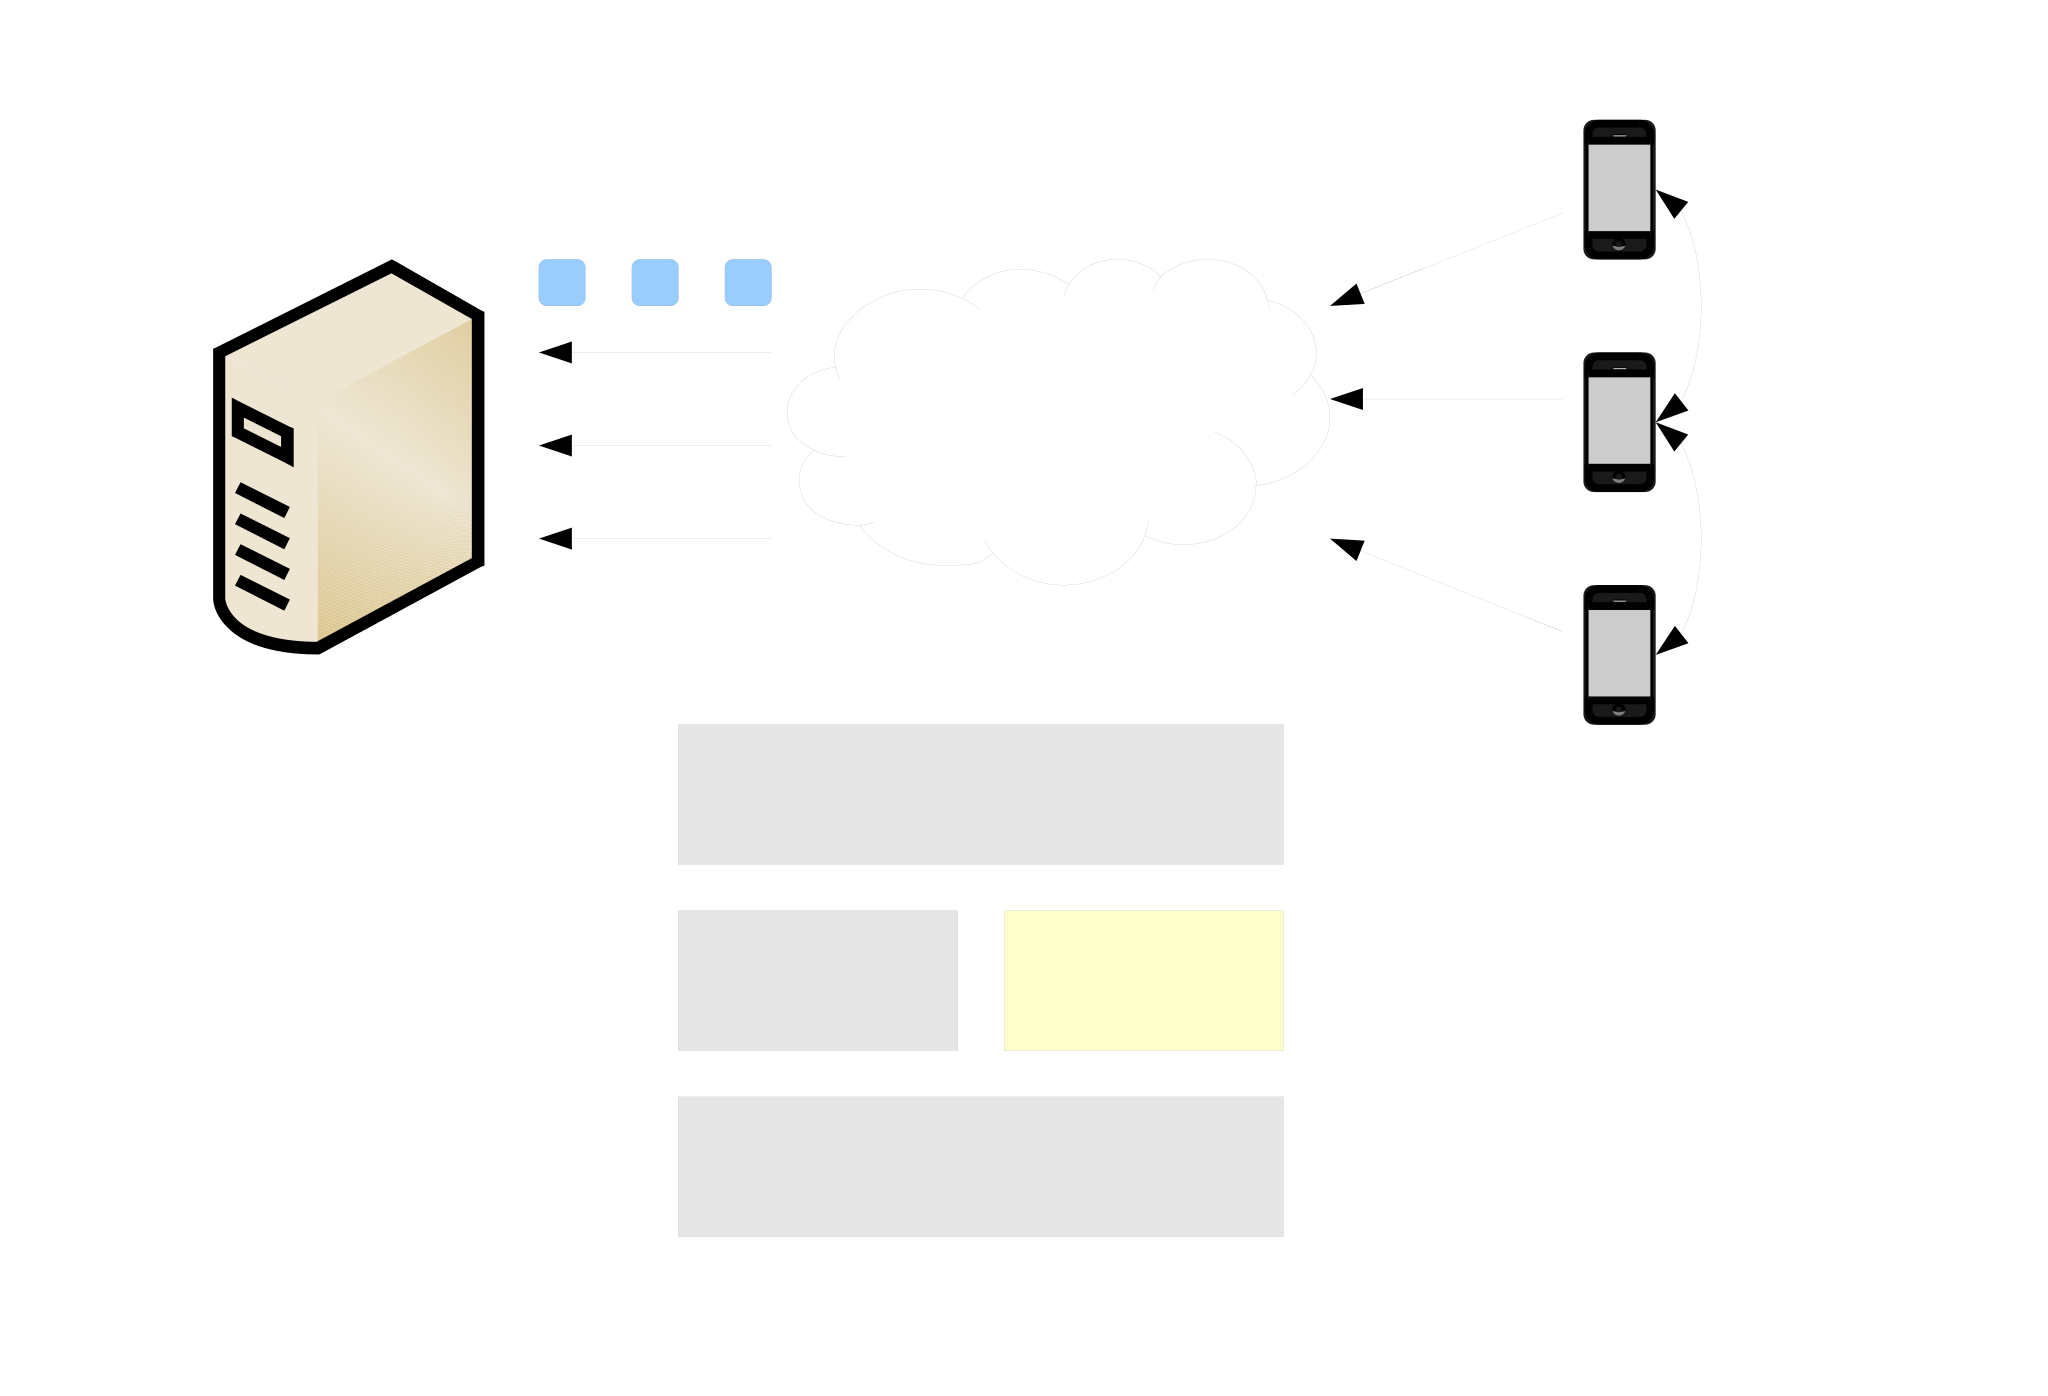
\includegraphics[width=3in]{figure1.eps}
\caption{\small \sl Anonymous Protocol.\label{fig:Stupendous}}
\end{center}
\end{figure}

What we would like is a protocol that completely removes the ownership and
source information from the data transmitted to the data collection server.
Figure 1 illustrates the concept of the theoretical anonymous One-Way
protocol.

We envision the protocol to be a network layer (layer 3) protocol that
replaces the IP protocol. The protocol will be very similar to the IP protocol
in the way that the packets includes the address of the destination host so
that the packets can be correct routed. The protocol should be able to
encapsulate upper layer (e.g. transport layer) data. The only difference is
that each packet does not include the address of the source host. In other
words, contractually, the client does not include the source address and the
server will have no access to the source information and thus keeping the
client's identity private.

Proponents might argue since the protocol resides on network layer (layer 3),
the source address could still be contained in the lower layer, e.g. the link
layer (layer 2). We argue that the source link address is different for
each hop on the route, and a route could easily contain 20 hops; therefore
the probability of tracing the link layer packet back to the original host is
really low.

%\begin{figure}[h]
%\begin{center}
%\includegraphics[width=3in]{arch.eps}
%\caption{\small \sl System Architecture.\label{fig:Stupendous}}
%\end{center}
%\end{figure}

\section{Anonymous Protocol Over Existing Protocols}\label{sec-protocol}
The One-Way protocol introduced in the previous section and Figure 1 is only
a theoretical protocol since it would take significant effort and drastic
change to current networking hardware infrastructure to introduce a new layer 3
routing protocol. In this section we modify the One-Way protocol depicted in
Figure 1 slightly so that it utilizes existing networking infrastructures. We
introduce two modifying approaches: tunneling and One-Way over User Datagram
Protocol (UDP).

\subsection{Tunneling}

In tunneling, the network topology is divided into two parts: a private
network that understands the One-Way protocol and the rest of the world that
only understand the IP protocol. The two parts are connected by the tunnel,
a special device, that does the translation between two routing protocols.

\begin{figure}[h]
\begin{center}
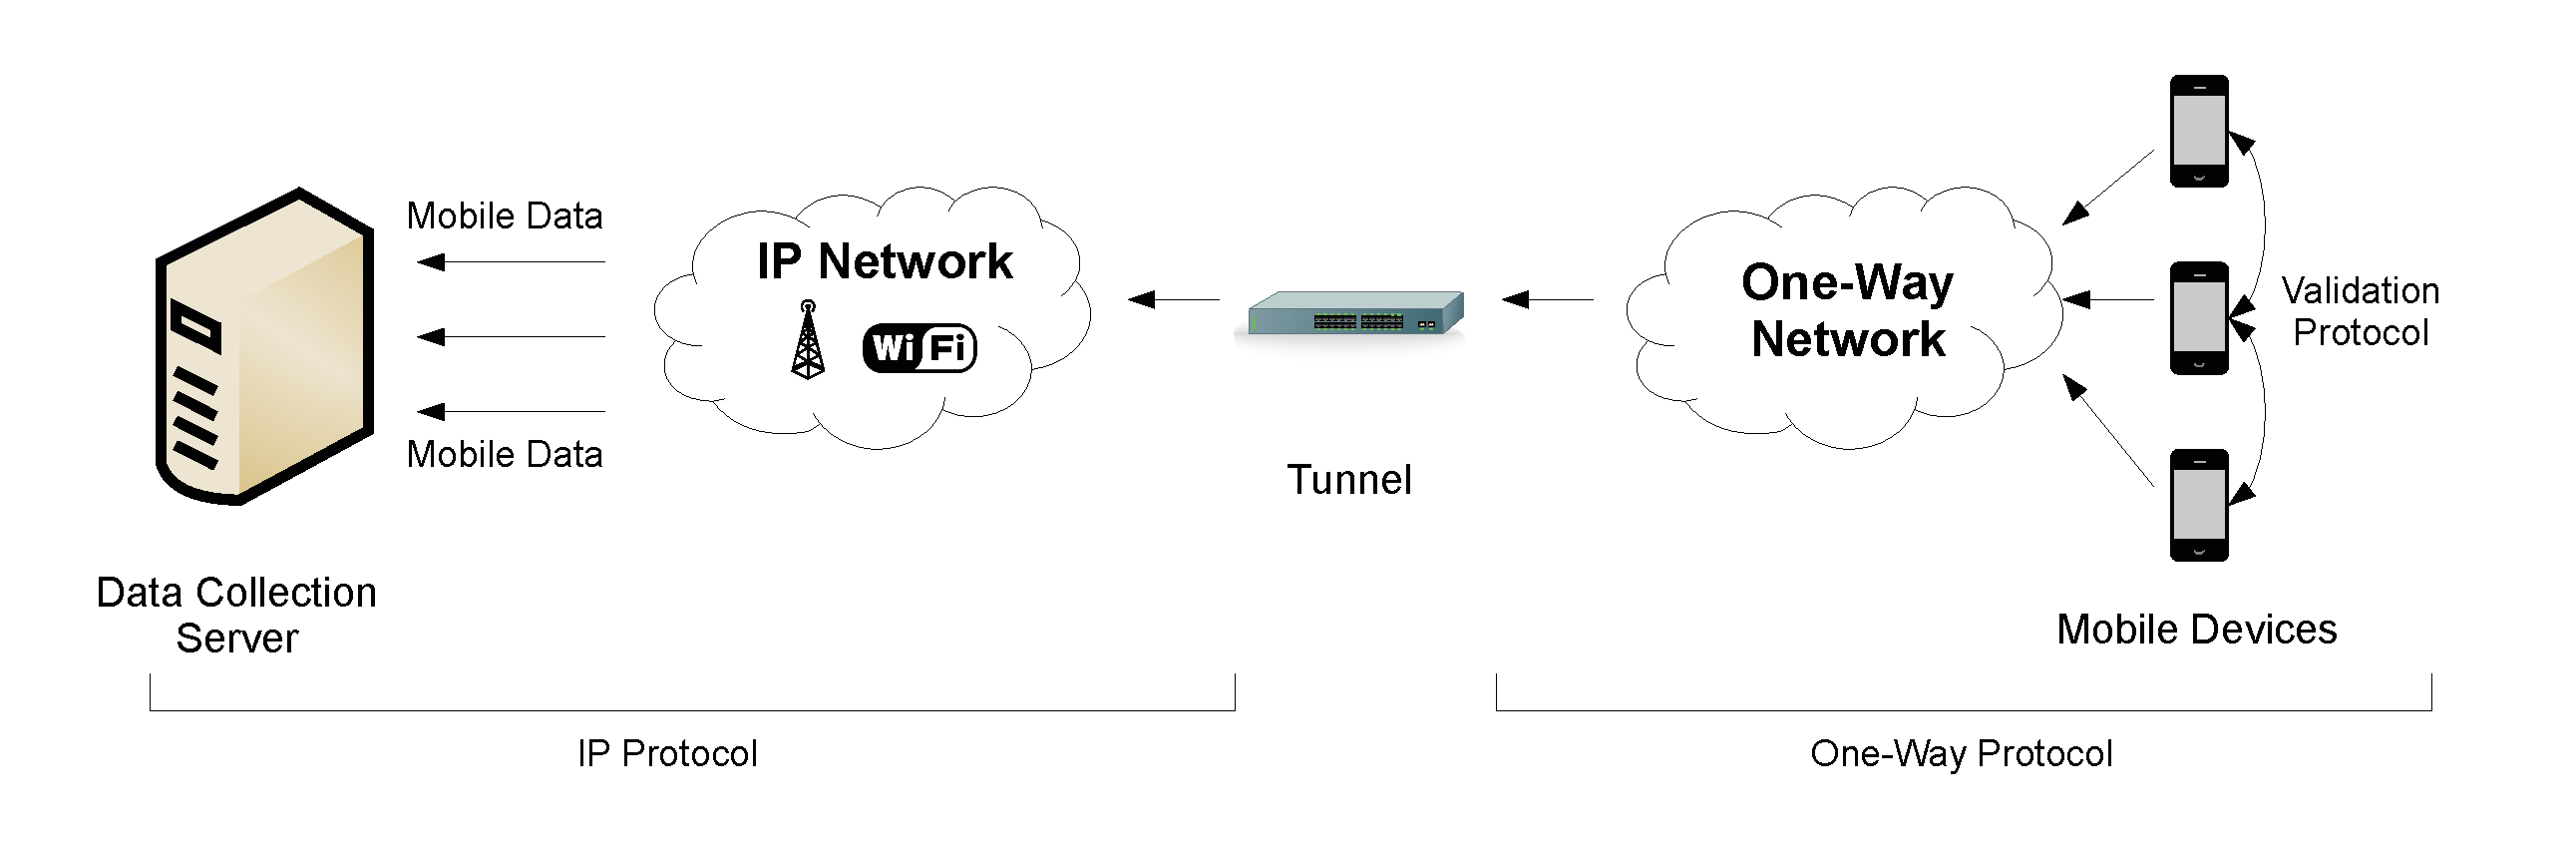
\includegraphics[width=3in]{figure2.eps}
\caption{\small \sl Tunneling.\label{fig:Stupendous}}
\end{center}
\end{figure}

\begin{figure}[h]
\begin{center}
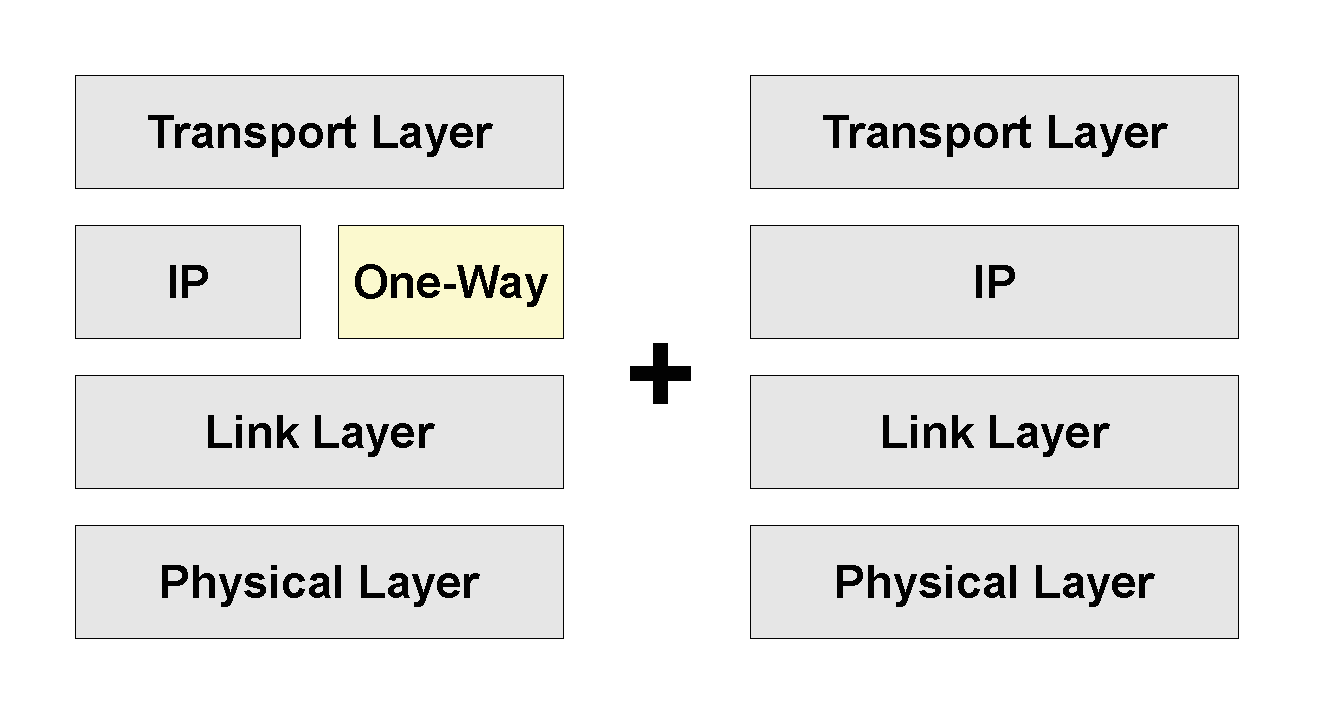
\includegraphics[width=3in]{figure2b.eps}
\caption{\small \sl Tunneling.\label{fig:Stupendous}}
\end{center}
\end{figure}

As illustrated in Figure 2, the tunneling device takes packets from the One-Way
network and forward the
data to the IP network. An important task of the tunneling device is to attach
source IP address to the packets that being forwarded. The device uses it own
IP address as the address of the packets and shields the identity of the mobile
clients. A reason for this tunneling approach is that some internet service
providers (ISP) will block packets without valid source host address. Figure 3
depicts the networking stack configuration of this approach. Tunneling is
similar to the Tor Anonymouse Protocol ~\cite{Tor}, in which clients sends data
through the designated Tor servers and the servers are responsible to deliver
the data to the destination.

Opponent could argument that attacker can still trace the mobile clients to a
specific subnet where the tunneling device resides. We argue that since most of
the clients are highly mobile, and with a number of tunneling device in one
geographic region, the identity of the mobile devices can be protected with high
confidence.

\subsection{Over User Datagram Protocol}
In this approach, we completely do away with a new routing protocol by building
the One-Way protocol as an application layer protocol on top of User Datagram
Protocol (UDP).

\begin{figure}[h]
\begin{center}
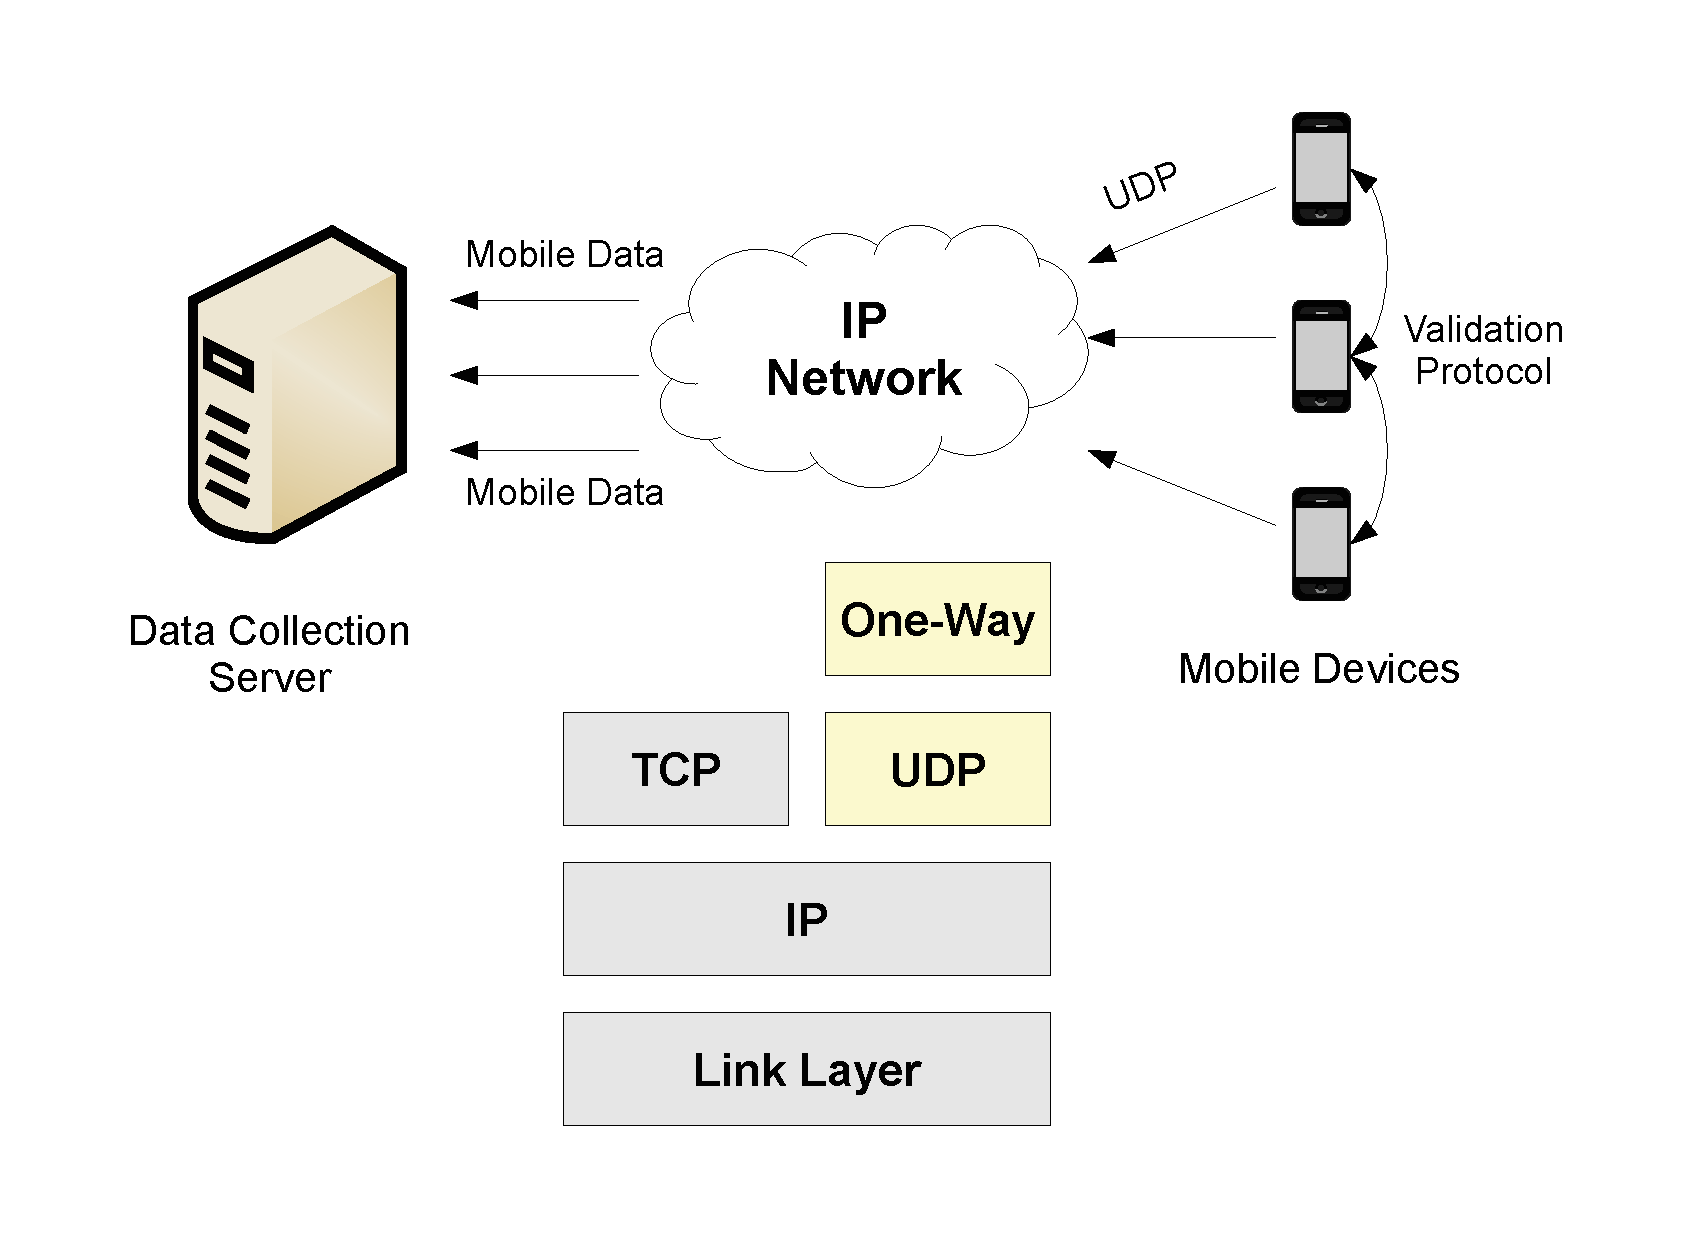
\includegraphics[width=3in]{figure4.eps}
\caption{\small \sl One-Way over UDP.\label{fig:Stupendous}}
\end{center}
\end{figure}

As illustrated in Figure 4, during transmission, the clients divides the data
into one or more UDP data packets, uses arbitrary IP address as the source
address -- to protect the identity of the mobile clients -- and sends the
packet into the network. The reason we use UDP instead of TCP is that since
the source IP is arbitrary, TCP will be unable to
establish a connection with the handshaking protocol.

In this setup, both the server and the clients need to implement the UDP One-Way
Protocol. The server has to be aware and to be able to reconstruct the complete
data from the fragments. In the future version of this protocol, we plan to
implement a protocol that allows the clients to verify that the data, in full,
has been successfully transmitted to the server.

In addition to running the protocol with no intermediate nodes, we can also combine
the UDP One-Way approach with the tunneling approach. Similar to what we described
in the previous subsection, the tunnel is an intermediate node that does translation
of protocols. The advantage of tunneling is that we can translate from UDP to TCP
protocol to provide reliable transmission. To do this kind of translation, the
tunnel create TCP packet from UDP packet and uses its own IP address as the source
address. An advantage of this translation is that the server does not necessarily
have to implement the One-Way protocol.

\subsection{Summary}
In this section we proposed an anonymous protocol that completely remove the source
address information of the data being transmitted. Three way to realize this protocol
are completely new protocol, new protocol over tunneling, and anonymous protocol
over UDP.

In the completely new protocol, we assume that we have complete freedom to implement
a new protocol and new network infrastructure. This is a very unrealistic and
impractical assumption, so we proposed new protocol and tunneling. In tunneling
we can implement the new One-Way protocol in our own small network and the tunnel
is responsible bridging our internal network and public IP network. In the UDP
approach, we build our new protocol on top of existing IP network, therefore
no new network infrastructure is required.

%In our experiment, we are able to send IP packets with arbitrary source address into
%the network and receive it on the server.


%\section{Related Work}\label{sec-relwork}
%\input{related}

%\section{System Architecture}\label{sec-design}
%\input{arch}

%\section{Experimental Validation}\label{sec-experiment}
%\input{experiments}

%\section{Conclusions}\label{sec-conc}
%\input{conc}

%\section{Acknowledgements}\label{sec-ack}
%\input{ack}


\setstretch{1}{
\bibliographystyle{plain}
\bibliography{Jeff_citations}
\end{document}
